 %%
%% Created in 2018 by Martin Slapak
%%
%% Based on file for NRP report LaTeX class by Vit Zyka (2008)
%%
%% Compilation:
%% >pdflatex report
%% >bibtex report
%% >pdflatex report
%% >pdflatex report

\documentclass[czech]{mvi-report}

\usepackage[utf8]{inputenc}
\usepackage{amsmath}
\usepackage{colortbl}
\usepackage{listings}
\usepackage{bm}

\usepackage{graphicx}
\graphicspath{ {./img/} }

\title{DÚ č.4 - Poissonův proces, systémy hromadné obsluhy}

\author{Marek Nevole, Jan Novotný}
\affiliation{ČVUT - FIT}
\email{\{nevolmar, novot103\}@fit.cvut.cz}

\def\file#1{{\tt#1}}

\begin{document}

\maketitle

%%%%%%%%%%%%%%%%%%%%%%%%%%%%%%%%%%%%%%%%%%%%%%%%%%%%%%%%%%%%%%%%%%%%%%%%%%%%%%%%
\section{Úvod}
Ve čtrtém úkolu z předmětu vybrané statistické metody jsme se zabývali Poissonovými procesy a systémy hromadné obsluhy. Za reprezentanta byl zvolen Marek Nevole.

Úkol jsme vypracovali pomocí programovacího jazyka Python\footnote{python.org} v prostředí Jupyter Notebook\footnote{jupyter.org} s volně dostupnými knihovnami SciPy\footnote{scipy.org}, NumPy\footnote{numpy.org}, Seaborn\footnote{seaborn.pydata.org} a Matplotlib\footnote{matplotlib.org}.

\section{Popis problému}
\textit{Uvažujte model hromadné obsluhy} $M$|$G$|$\infty$.
\begin{itemize}
  \item \textit{Požadavky přichází podle Poissonova procesu s intenzitou $\lambda = 10~\mathrm{s}^{-1}$.}
  \item \textit{Doba obsluhy jednoho požadavku (v sekundách) má rozdělení $S\sim\mathrm{Ga}(4,2)$, tj. Gamma s parametry $a = 4, p = 2$.}
  \item \textit{Časy mezi příchody a časy obsluhy jsou nezávislé.}
  \item \textit{Systém má (teoreticky) nekonečně paralelních obslužných míst (každý příchozí je rovnou obsluhován).}
\end{itemize}
\textit{Označme $N_t$ počet zákazníků v systému v čase $t$. Předpokládejme, že na začátku je systém prázdný, tj. $N_0 = 0$.}


\section{Úloha č.1}
\textit{Simulujte jednu trajektorii $\{N_t(\omega) \mid t\in(0,10~\mathrm{s})\}$. Průběh trajektorie graficky znázorněte.}\\

Zákazníci přichází podle Poissonova procesu s intenzitou $ \lambda = 10~s^{-1} $. Počet příchozích zákazníků v intervalu $ [s,t] $ odpovídá Poissonovu rozdělení přírůstků $ N_t - N_s \sim \textrm{Poisson}(\lambda (t-s)) $, tedy počet zákazníků této úlohy je z rozdělení $ \textrm{Poisson}(100) $. Toto rozdělení je implementováno v knihovně SciPy jako \textit{poisson} a pro náhodný výběr obsahuje metodu \textit{rvs}, které jsme předali parametr \textit{mu=100}. Náhodný výběr z tohoto rozdělení vrátil hodnotu $  n=95 $. Časy jednotlivých příchodů zákazníků odpovídají rovnoměrnému rozdělení $ U(0,t) $. Tedy jsme udělali 95 náhodných výběrů z rozdělení $ U(0,10) $, pomocí třídy \textit{uniform} a metody \textit{rvs} s parametry \textit{scale=t, size=n}. Doba obsloužení těchto zákazníků je z rozdělení $\mathrm{Ga}(4,2)$ s parametry $ a = 4, p = 2 $. Gamma rozdělení je implementováno jako \textit{gamma} s metodou pro náhodný výběr \textit{rvs}. Parametry pro tuto metodu jsou \textit{shape} a \textit{scale}, v našem studijním textu používáme parametry, které odpovídají parametrizaci \textit{shape} a \textit{rate}. Pro $ \mathrm{Ga}(a,p) $ je \textit{shape} = p a \textit{rate} = a. Mezi \textit{scale} a \textit{rate} lze převádět pomocí vzorce $\mathrm{scale}=\frac{1}{\mathrm{rate}} $. Tedy po 95 náhodných výběrech z $\mathrm{Ga}(4,2)$ jsme dostali intervaly všech zákazníků v čase a výslednou trajektorii lze pozorovat na obrázku \ref{fig:traj}.

\begin{figure}
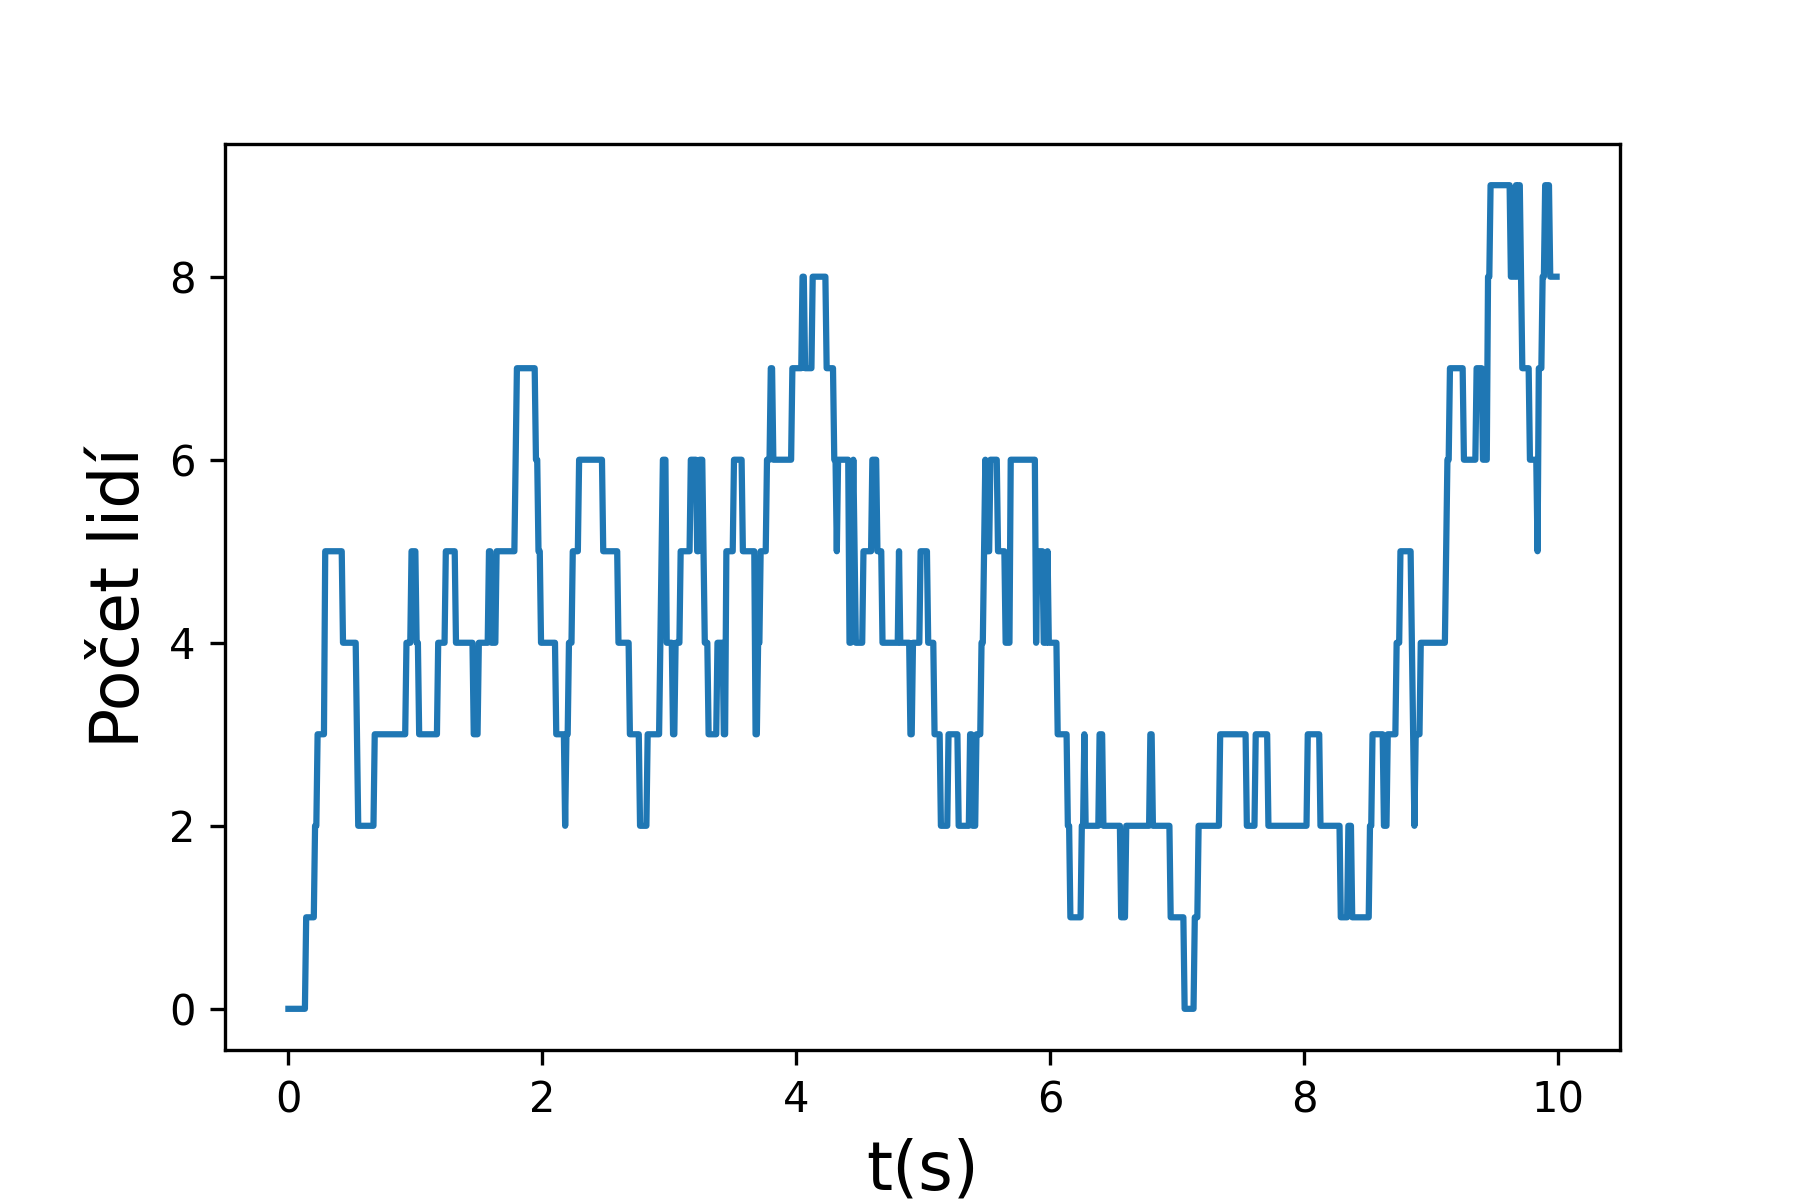
\includegraphics[width=\columnwidth]{img/traj.png} 
\caption{Jedna trajektorie $ \{N_t(\omega) \mid t\in(0,10~\mathrm{s})\} $.}
\label{fig:traj}
\end{figure}

\section{Úloha č.2}
\textit{Simulujte $n = 500$ nezávislých trajektorií pro $t\in(0,100)$. Na základě těchto simulací odhadněte rozdělení náhodné veličiny $N_{100}$.}\\

V této úloze jsme využili kód z předchozí úlohy a simulovali jsme 500 trajektorií. Na základě hodnot z posledního časového kroku, tedy v $ t=100 $, jsme sestavili histogram a  odhad hustoty rozdělení pomocí jádrového odhadu, toto lze pozorovat na obrázku \ref{fig:histkde}.

\begin{figure}
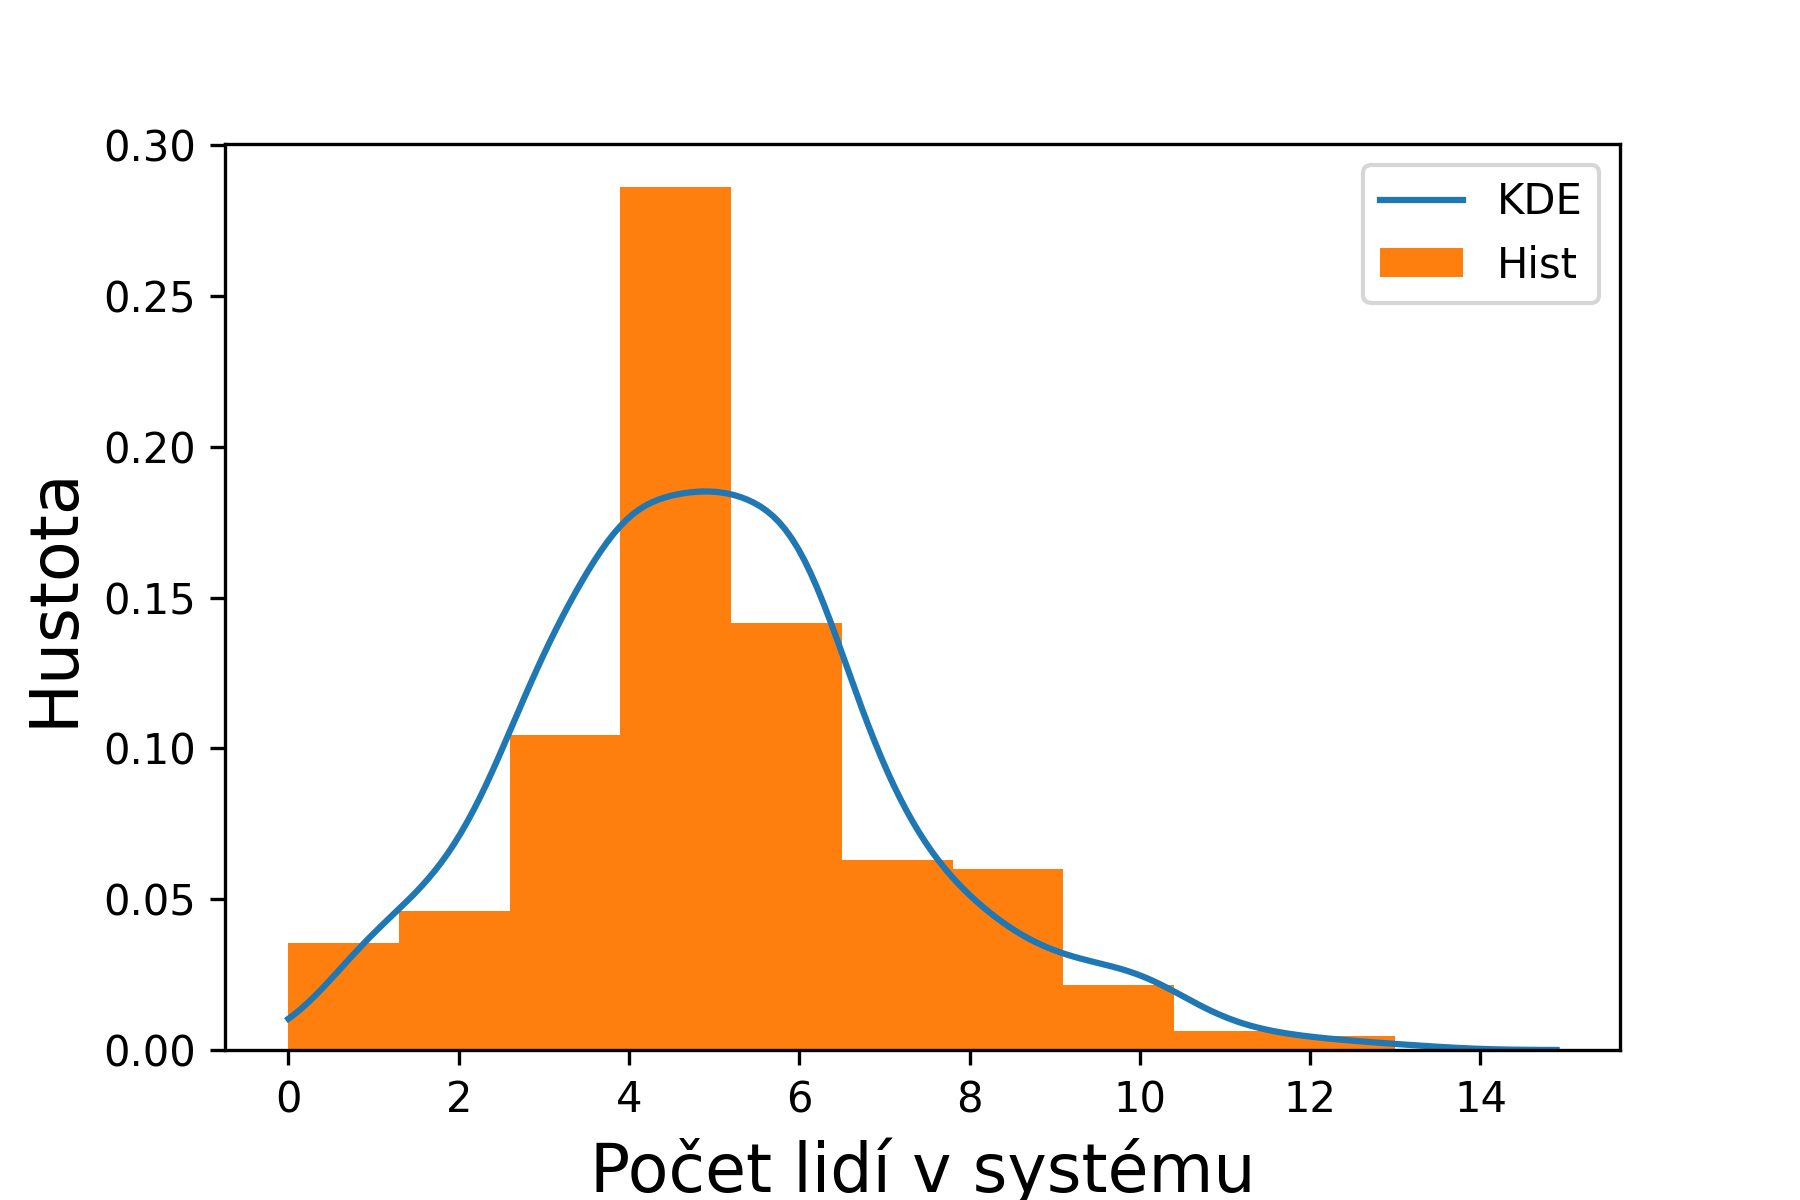
\includegraphics[width=\columnwidth]{img/histkde.png} 
\caption{ Odhad rozdělení $ N_{100} $ pomocí histogramu a jádrového odhadu.}
\label{fig:histkde} 
\end{figure}

\section{Úloha č.3}
\textit{Diskutujte, jaké je limitní rozdělení tohoto systému pro $t\to+\infty$. Pomocí vhodného testu otestujte na hladině významnosti 5~\%, zda výsledky simulace $N_{100}$ odpovídají tomuto rozdělení.}\\

\end{document}